\documentclass[t,10pt,serif,professionalfonts]{beamer}

\mode<presentation>{
  \usetheme{goudie}
  \usecolortheme{goudie}
}

\usepackage{amsmath, amsthm, amssymb, mathtools, multirow, dsfont, color, graphicx, lscape, units, tikz, booktabs, fixltx2e, bbm, ulem, setspace, MinionPro, MnSymbol}

\setstretch{1.25}
\setlength{\ULdepth}{0.4em}
\normalem

\usepackage[backend=biber,firstinits=true,style=authoryear,doi=false,url=false,alldates=year]{biblatex}
\DeclareNameAlias{default}{last-first}
\DeclareNameAlias{sortname}{last-first}
% hide month and number, and make volume bold
\AtEveryBibitem{\clearfield{number}}%
\AtEveryCitekey{\clearfield{number}}%
\DeclareFieldFormat[article]{volume}{\mkbibbold{#1}}%
\renewbibmacro{in:}{\ifentrytype{article}{}{\printtext{\bibstring{in}\intitlepunct}}}%
\DeclareFieldFormat[article]{pages}{#1}%

\bibliography{../../../documents/bib/offline,../../../documents/bib/papers}

\let\oldfootnote\footnote
\renewcommand\footnote[1][]{\oldfootnote[frame,#1]}

\usetikzlibrary{calc, fit, positioning, shapes, arrows}
\tikzset{>={stealth}}

% symbols
\def\ci{\perp\!\!\!\perp} % from Wikipedia
\def\notci{\perp\!\!\!\perp\!\!\!\!\!\!\!\!\!\!\;\diagup\;} % from Wikipedia

% Distributions
\newcommand{\dunif}{\text{U}}
\newcommand{\dgamma}{\text{Gam}}
\newcommand{\dinvgamma}{\text{Inv-Gam}}
\newcommand{\dwishart}{\text{Wishart}}
\newcommand{\dinvwishart}{\text{Inv-Wishart}}
\newcommand{\dmult}{\text{Mult}}
\newcommand{\dnorm}{\text{N}}
\newcommand{\dmvnorm}{\text{MVN}}
\newcommand{\dlnorm}{\text{Lognormal}}
\newcommand{\dbin}{\text{Bin}}
\newcommand{\dpoi}{\text{Po}}
\newcommand{\dbeta}{\text{Beta}}

% General
\newcommand{\den}{p}
\newcommand{\prior}{\pi}
\newcommand{\mydiff}[1]{\, \text{d}#1}
\newcommand{\indicator}[1]{\, \mathbbm{1}_{#1}}
\newcommand{\given}{\mid}
\newcommand{\distributedas}{\sim}
\newcommand{\function}{f}
\newcommand{\vect}[1]{\left(#1\right)}
\newcommand{\set}[1]{\{\,#1\,\}}
\newcommand{\suchthat}{:}

\begin{document}

\title{Title of talk}
\author{Robert Goudie}
\date{\today}
\maketitle

\begin{frame}
\frametitle{Notation}

abc
\bigskip
def

\end{frame}

\begin{frame}{DAG representation}

\vfill
\centering
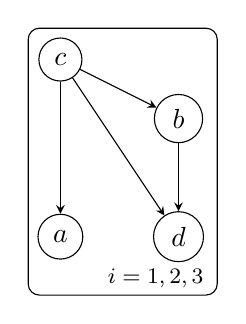
\begin{tikzpicture}
\node[circle, draw] (select) at (0, 0.75) {\(a\)};
\node[circle, draw] (covariates) at (1.5, 2.25) {\(b\)};
\node[circle, draw] (design) at (0, 3) {\(c\)};
\node[circle, draw] (outcome) at (1.5, 0.75) {\(d\)};

\draw[->] (design) -- (select);
\draw[->] (design) -- (covariates);
\draw[->] (design) -- (outcome);
\draw[->] (covariates) -- (outcome);

\node (dummy) at (1.75, 0.25) {};

\node[draw, rectangle, rounded corners,
      fit={(select) (covariates) (design) (outcome) (dummy)}] (plate) {};
\node[font = \footnotesize, node distance=0, inner sep=0pt, below left=-10pt and 5pt of plate.south east] {\(i = 1, 2, 3\)};
\end{tikzpicture}
\vfill
\end{frame}

\begin{frame}[fragile]{Sampling scenarios}
There are various possible sampling scenarios \footfullcite{Chambers:2003}, including

\begin{itemize}
\item Also \footfullcite{OMalley:2008ch}

\item And\footfullcite{Richardson:2016dv}
\end{itemize}
\end{frame}

\end{document}
